\documentclass{article}
\usepackage{amsmath}
\usepackage[margin=0.5in]{geometry}
\usepackage[utf8]{inputenc}
\usepackage{textcomp}
\usepackage{pgfplots}
\pgfplotsset{width=10cm,compat=1.9}
\usepackage{pdfcomment}
\usepackage{textcomp}

\usepackage[tagged]{accessibility}
\begin{document}

   
 f Open Parenthesis x Close Parenthesis  is equal to   fraction numerator p Open Parenthesis x Close Parenthesis  . . .  over  denominator q Open Parenthesis x Close Parenthesis  . . .  end Frac . . .  
\\
\\

More plain text.
\\  



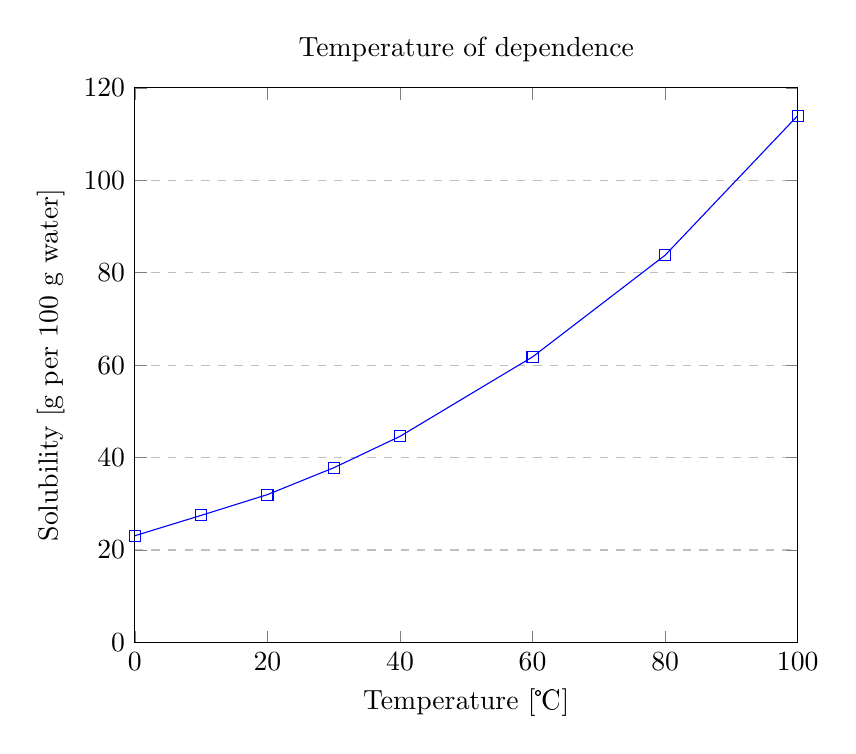
\begin{tikzpicture}
\begin{axis}[
    title={Temperature of dependence},
    xlabel={Temperature [\textcelsius]},
    ylabel={Solubility [g per 100 g water]},
    xmin=0, xmax=100,
    ymin=0, ymax=120,
    xtick={0,20,40,60,80,100},
    ytick={0,20,40,60,80,100,120},
    legend pos=north west,
    ymajorgrids=true,
    grid style=dashed,
]
\addplot[
    color=blue,
    mark=square,
    ]
    coordinates {
    (0,23.1)(10,27.5)(20,32)(30,37.8)(40,44.6)(60,61.8)(80,83.8)(100,114)
    };
     
\end{axis}

\end{tikzpicture}

 
\end{document}

